\setbeamerfont{block title}{size=\scriptsize}

\section{Analyzing the build}

\begin{frame}{Analyzing the build: available tools}
  \begin{itemize}
  \item Buildroot provides several useful tools to analyze the build:
    \begin{itemize}
    \item The {\bf licensing report}, covered in a previous section,
      which allows to analyze the list of packages and their licenses.
    \item The {\bf dependency graphing} tools
    \item The {\bf build time graphing} tools
    \item The {\bf filesystem size} tools
    \end{itemize}
  \item Additional tools can be constructed using {\bf instrumentation
      scripts}
  \end{itemize}
\end{frame}

\begin{frame}{Dependency graphing}
  \begin{itemize}
  \item Exploring the dependencies between packages is useful to
    understand
    \begin{itemize}
    \item why a particular package is being brought into the
      build
    \item if the build size and duration can be reduced
    \end{itemize}
  \item \code{make graph-depends} to generate a full dependency graph,
    which can be huge!
  \item \code{make <pkg>-graph-depends} to generate the dependency
    graph of a given package
  \item The graph is done according to the current Buildroot
    configuration.
  \item Resulting graphs in \code{$(O)/graphs/}
  \end{itemize}
\end{frame}

\begin{frame}{Dependency graph example}
  \begin{center}
    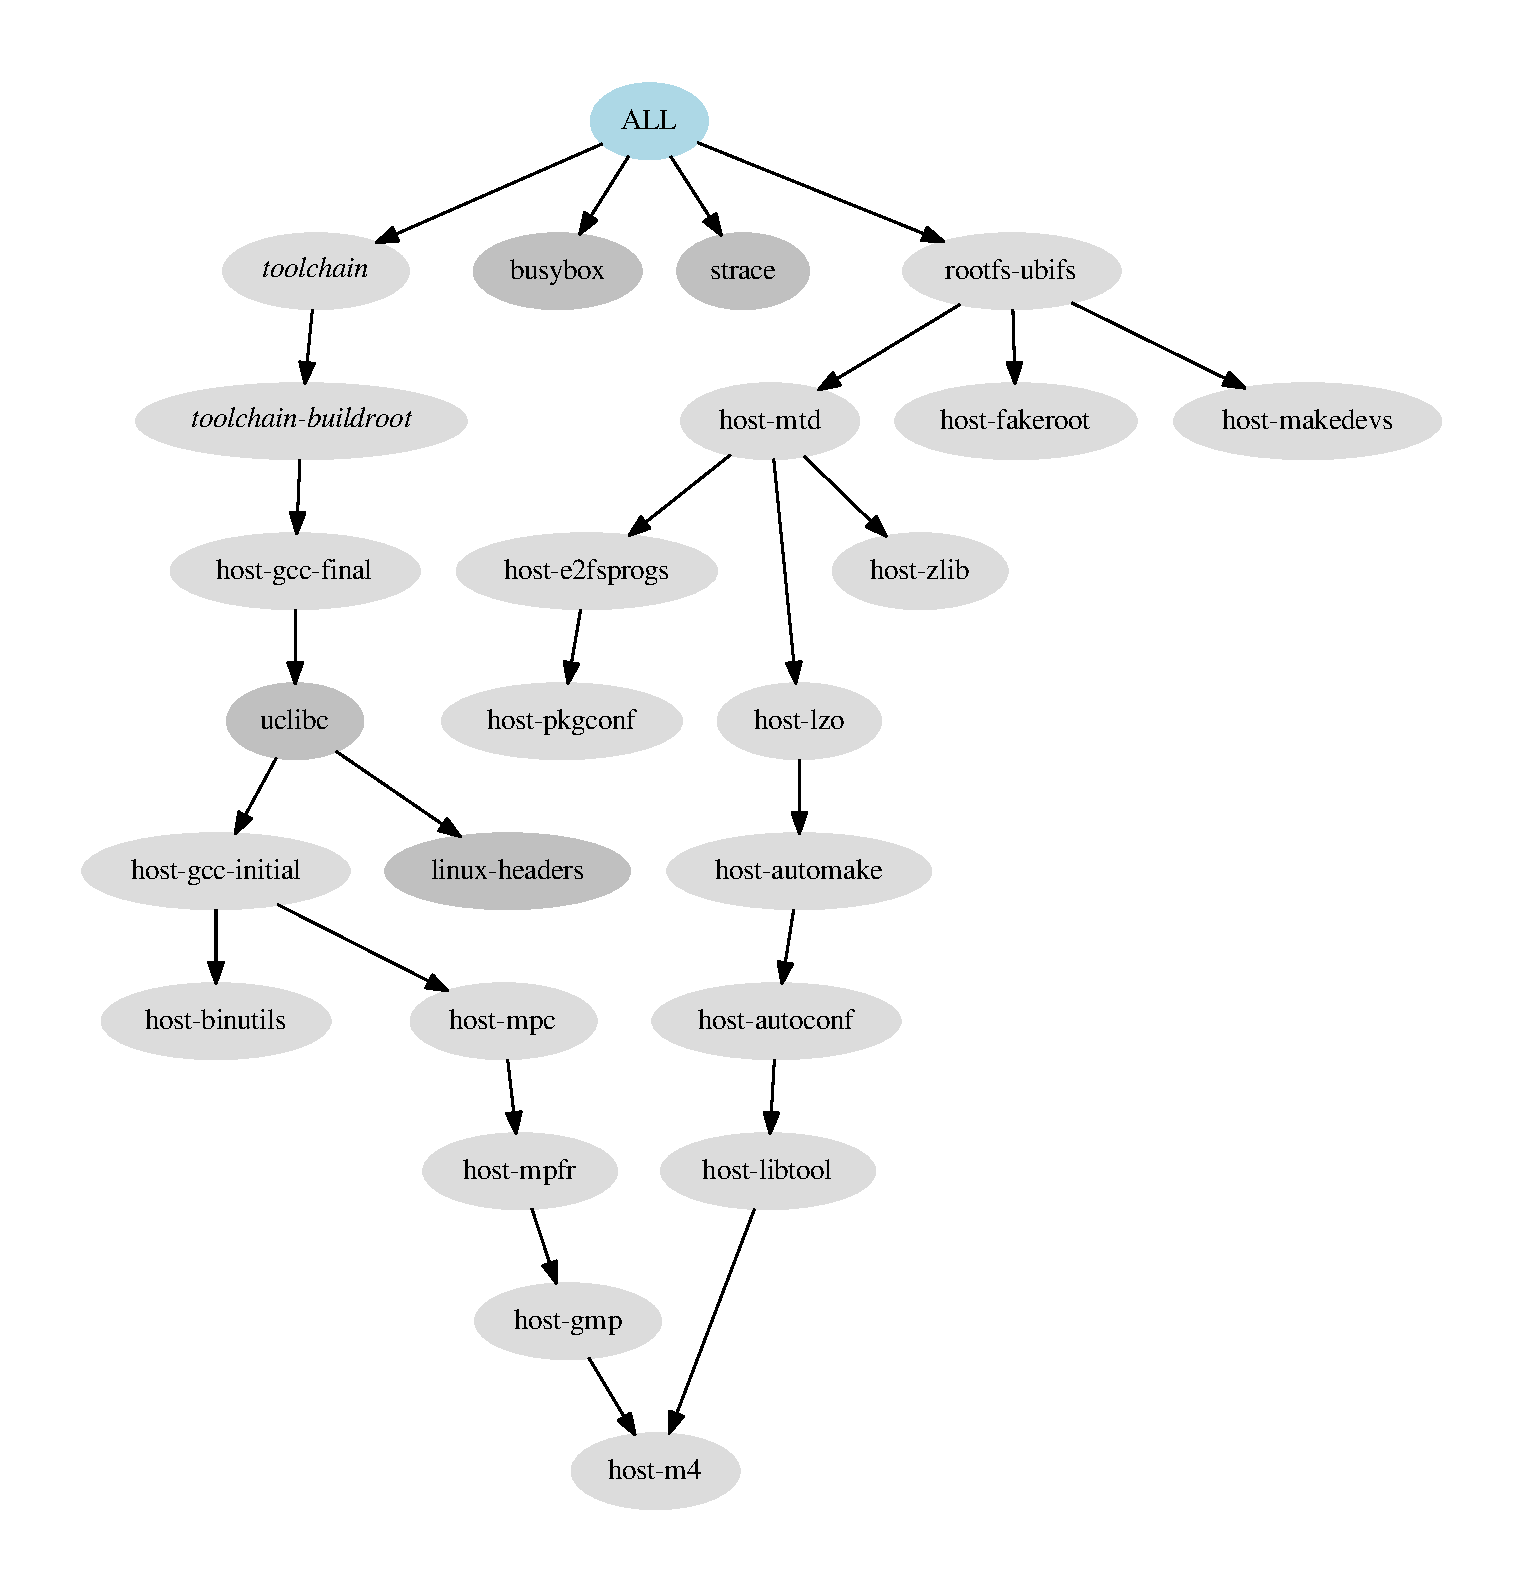
\includegraphics[height=0.8\textheight]{slides/buildroot-analysis/graph-depends.pdf}
  \end{center}
\end{frame}

\begin{frame}[fragile]{Dependency graphing: advanced}
  \begin{itemize}
  \item Variable \code{BR2_GRAPH_OUT}, to select the output
    format. Defaults to \code{pdf}, can be \code{png} or \code{svg}
    for example.
  \item Internally, the graph is generated by the Python script
    \code{support/scripts/graph-depends}
  \item All options that this script supports can be passed using the
    \code{BR2_GRAPH_DEPS_OPTS} variable when calling \code{make
      graph-depends}
  \item Example
    \begin{itemize}
    \item Generate a PNG graph of the \code{openssh} package
      dependencies
    \item Custom colors
    \item Stop graphing on the \code{host-automake} package, to remove
      a part of the graph we're not interested in
    \end{itemize}
  \end{itemize}

  \begin{block}{}
{\tiny
\begin{verbatim}
BR2_GRAPH_OUT=png \
    BR2_GRAPH_DEPS_OPTS="--colours red,blue,green --stop-on=host-automake" \
    make openssh-graph-depends
\end{verbatim}}
  \end{block}
\end{frame}

\begin{frame}{Build time graphing}
  \begin{itemize}
  \item When the generated embedded Linux system grows bigger and
    bigger, the build time also increases.
  \item It is sometimes useful to analyze this build time, and see if
    certain packages are particularly problematic.
  \item Buildroot collects build duration data in the file
    \code{$(O)/build/build-time.log}
  \item \code{make graph-build} generates several graphs in
    \code{$(O)/graphs/}:
    \begin{itemize}
    \item \code{build.hist-build.pdf}, build time in build order
    \item \code{build.hist-duration.pdf}, build time by duration
    \item \code{build.hist-name.pdf}, build time by package name
    \item \code{build.pie-packages.pdf}, pie chart of the per-package
      build time
    \item \code{build.pie-steps.pdf}, pie chart of the per-step build
      time
    \end{itemize}
  \item Note: only works properly after a complete clean rebuild.
  \end{itemize}
\end{frame}

\begin{frame}{Build time graphing: example}
  \begin{center}
    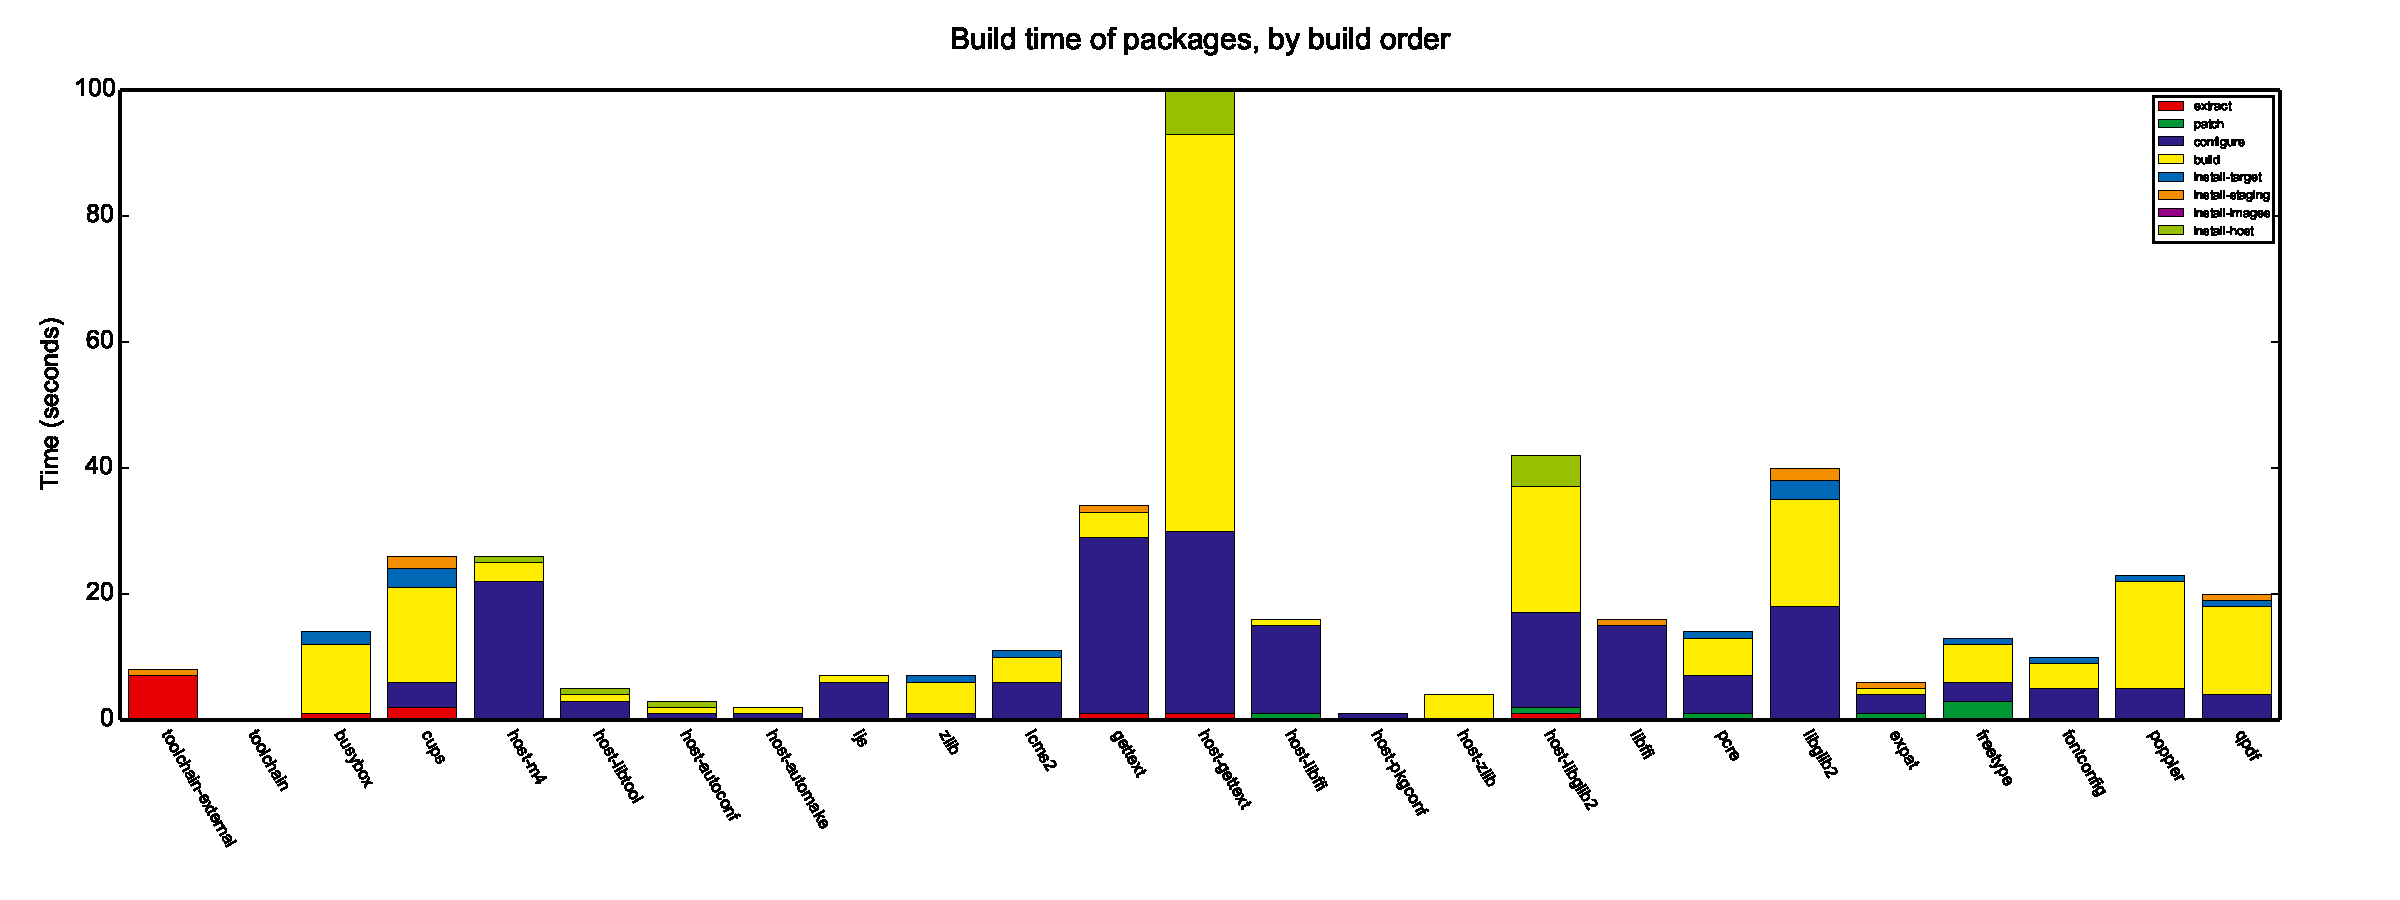
\includegraphics[width=\textwidth]{slides/buildroot-analysis/build-hist-build.pdf}
  \end{center}
\end{frame}

\begin{frame}{Filesystem size graphing}
  \begin{itemize}
  \item In many embedded systems, storage resources are limited.
  \item For this reason, it is useful to be able to analyze the size
    of your root filesystem, and see which packages are consuming the
    biggest amount of space.
  \item Allows to focus the size optimizations on the relevant
    packages.
  \item Buildroot collects data about the size installed by each
    package.
  \item \code{make graph-size} produces:
    \begin{itemize}
    \item \code{file-size-stats.csv}, CSV with the raw data of the
      per-file size
    \item \code{package-size-stats.csv}, CSV with the raw data of the
      per-package size
    \item \code{graph-size.pdf}, pie chart of the per-package size
      consumption
    \end{itemize}
  \end{itemize}
\end{frame}

\begin{frame}{Filesystem size graphing: example}
  \begin{center}
    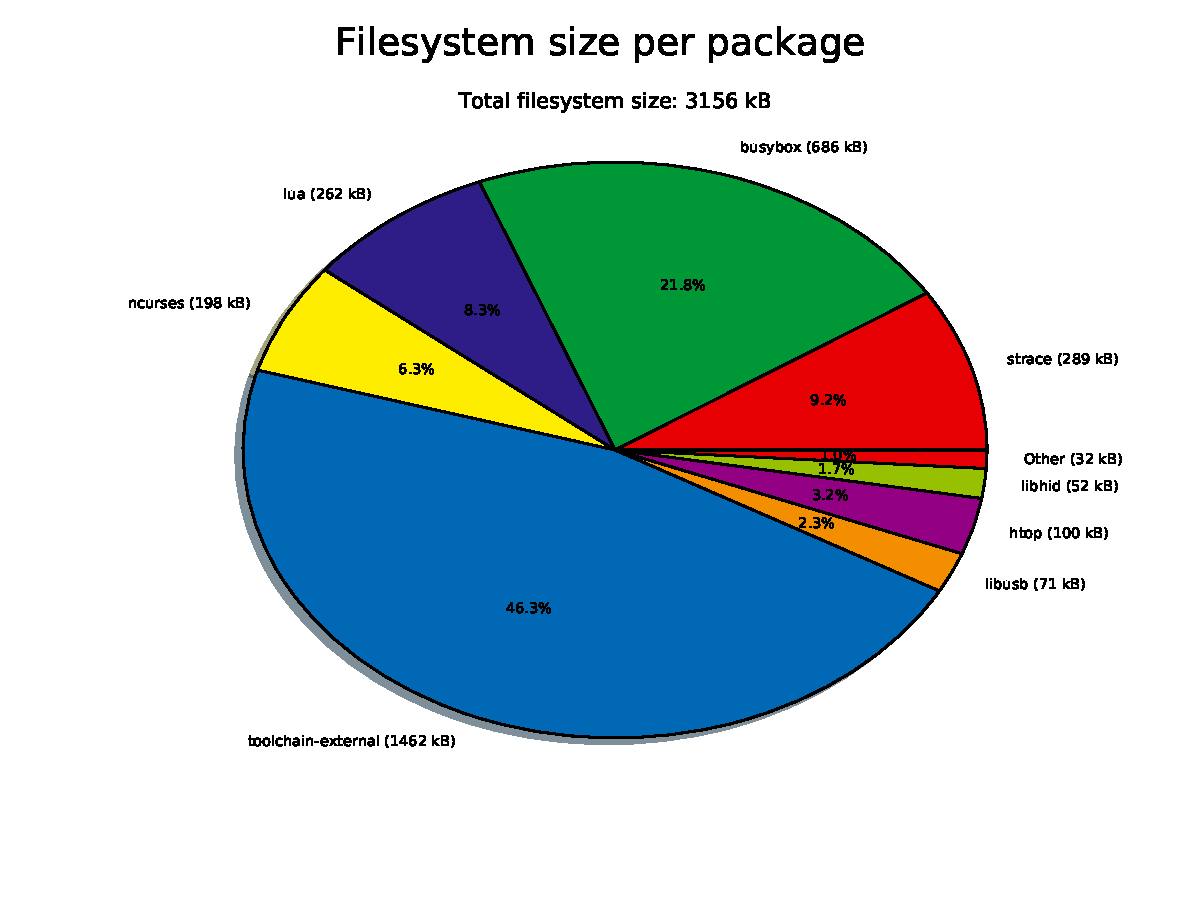
\includegraphics[height=0.8\textheight]{slides/buildroot-analysis/graph-size.pdf}
  \end{center}
\end{frame}

\begin{frame}{Instrumentation scripts}
  \begin{itemize}
  \item Additional analysis tools can be constructed using the {\bf
      instrumentation scripts} mechanism.
  \item \code{BR2_INSTRUMENTATION_SCRIPTS} is an environment variable,
    containing a space-separated list of scripts, that will be called
    before and after each step of the build of all packages.
  \item Three arguments are passed to the scripts:
    \begin{enumerate}
    \item \code{start} or \code{stop} to indicate whether it's the
      beginning or end of the step
    \item the name of the step
    \item the name of the package
    \end{enumerate}
  \end{itemize}
\end{frame}

\begin{frame}[fragile]{Instrumentation scripts: example}
  \begin{block}{instrumentation.sh}
{\tiny
\begin{verbatim}
#!/bin/sh
echo "${3} now ${1}s ${2}"
\end{verbatim}}
  \end{block}

  \begin{block}{Output}
{\tiny
\begin{verbatim}
$ make BR2_INSTRUMENTATION_SCRIPTS="./instrumentation.sh"
strace now starts extract
>>> strace 4.10 Extracting
xzcat /home/thomas/dl/strace-4.10.tar.xz | tar --strip-components=1 \
      -C /home/thomas/projets/buildroot/output/build/strace-4.10  -xf -
strace now ends extract
strace now starts patch
>>> strace 4.10 Patching

Applying 0001-linux-aarch64-add-missing-header.patch using patch: 
patching file linux/aarch64/arch_regs.h
>>> strace 4.10 Updating config.sub and config.guess
for file in config.guess config.sub; do for i in $(find \
    /home/thomas/projets/buildroot/output/build/strace-4.10 -name $file); do \
       cp support/gnuconfig/$file $i; done; done
>>> strace 4.10 Patching libtool
strace now ends patch
strace now starts configure
>>> strace 4.10 Configuring
\end{verbatim}}
  \end{block}

\end{frame}

